\subsection{sacabench list}
\label{framework:cli:sacabench-list}

{
\begin{wrapfigure}[12]{R}[5mm]{.5\textwidth}
    \vspace{-1.5\baselineskip}
    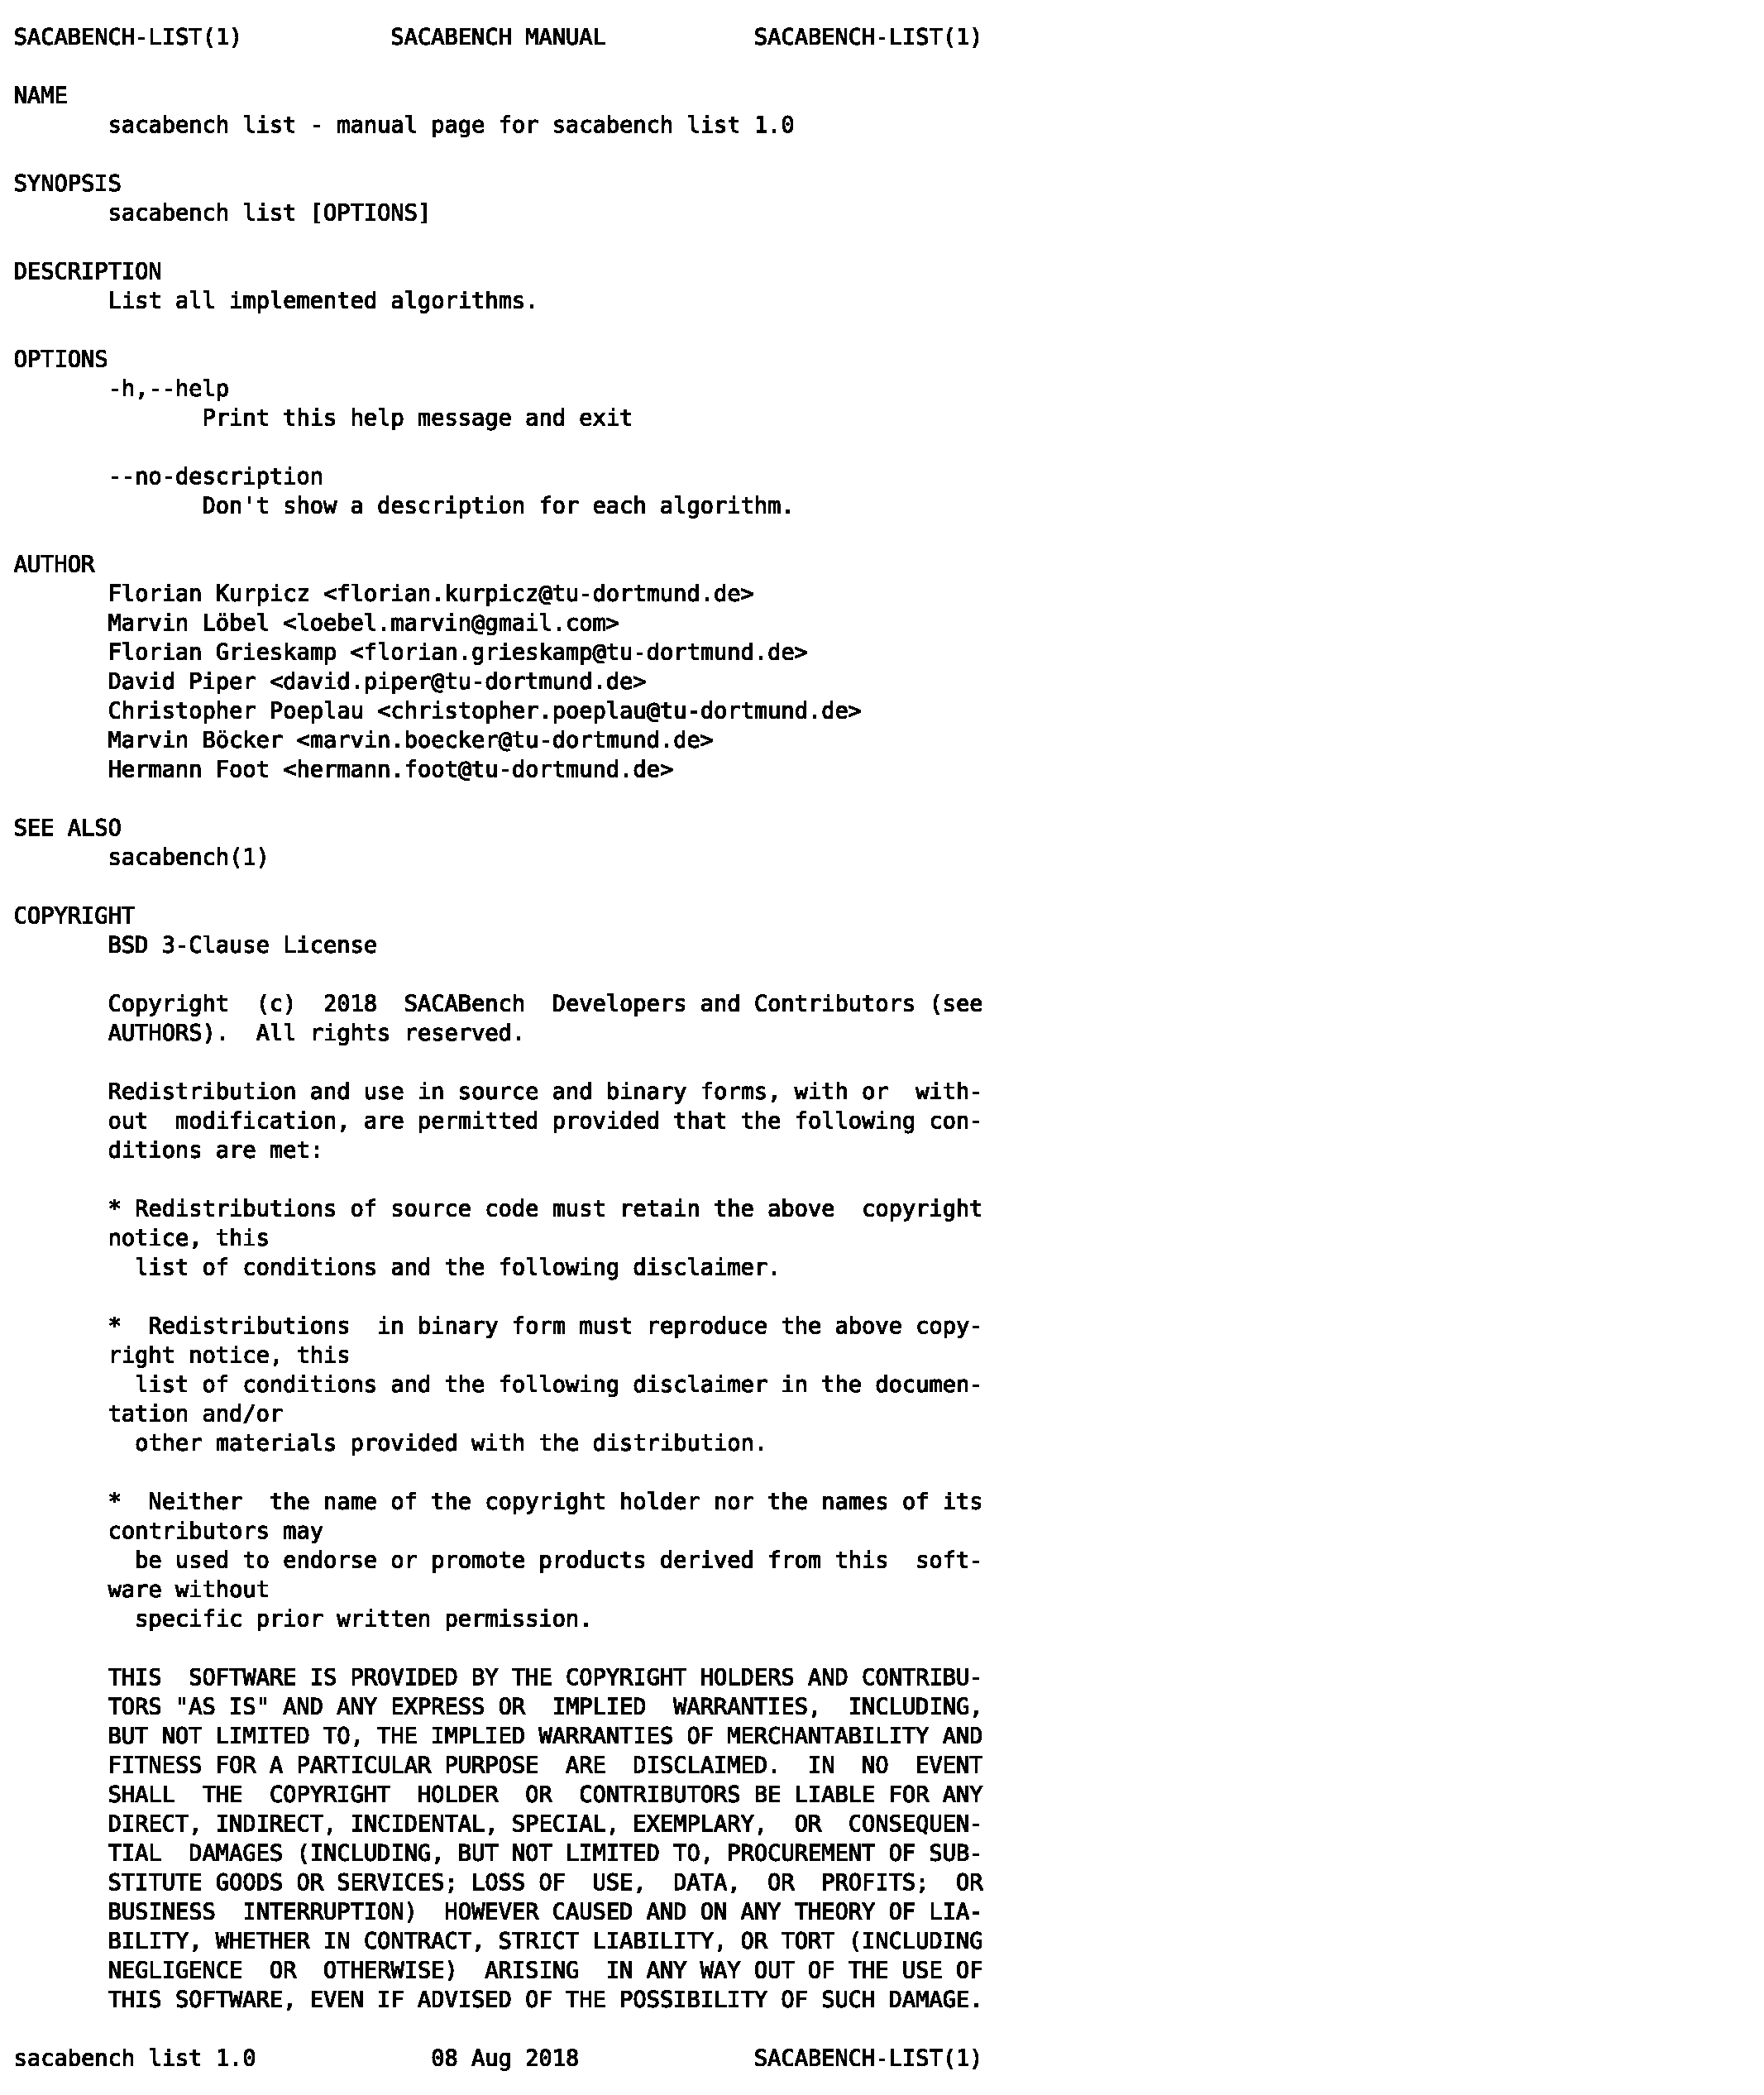
\includegraphics[page=1, viewport=0cm 32.8cm 20.5cm 42.5cm, clip, width=.5\textwidth]{{kapitel/3_framework/cli/sacabench-list/sacabench-list}.pdf}\\
    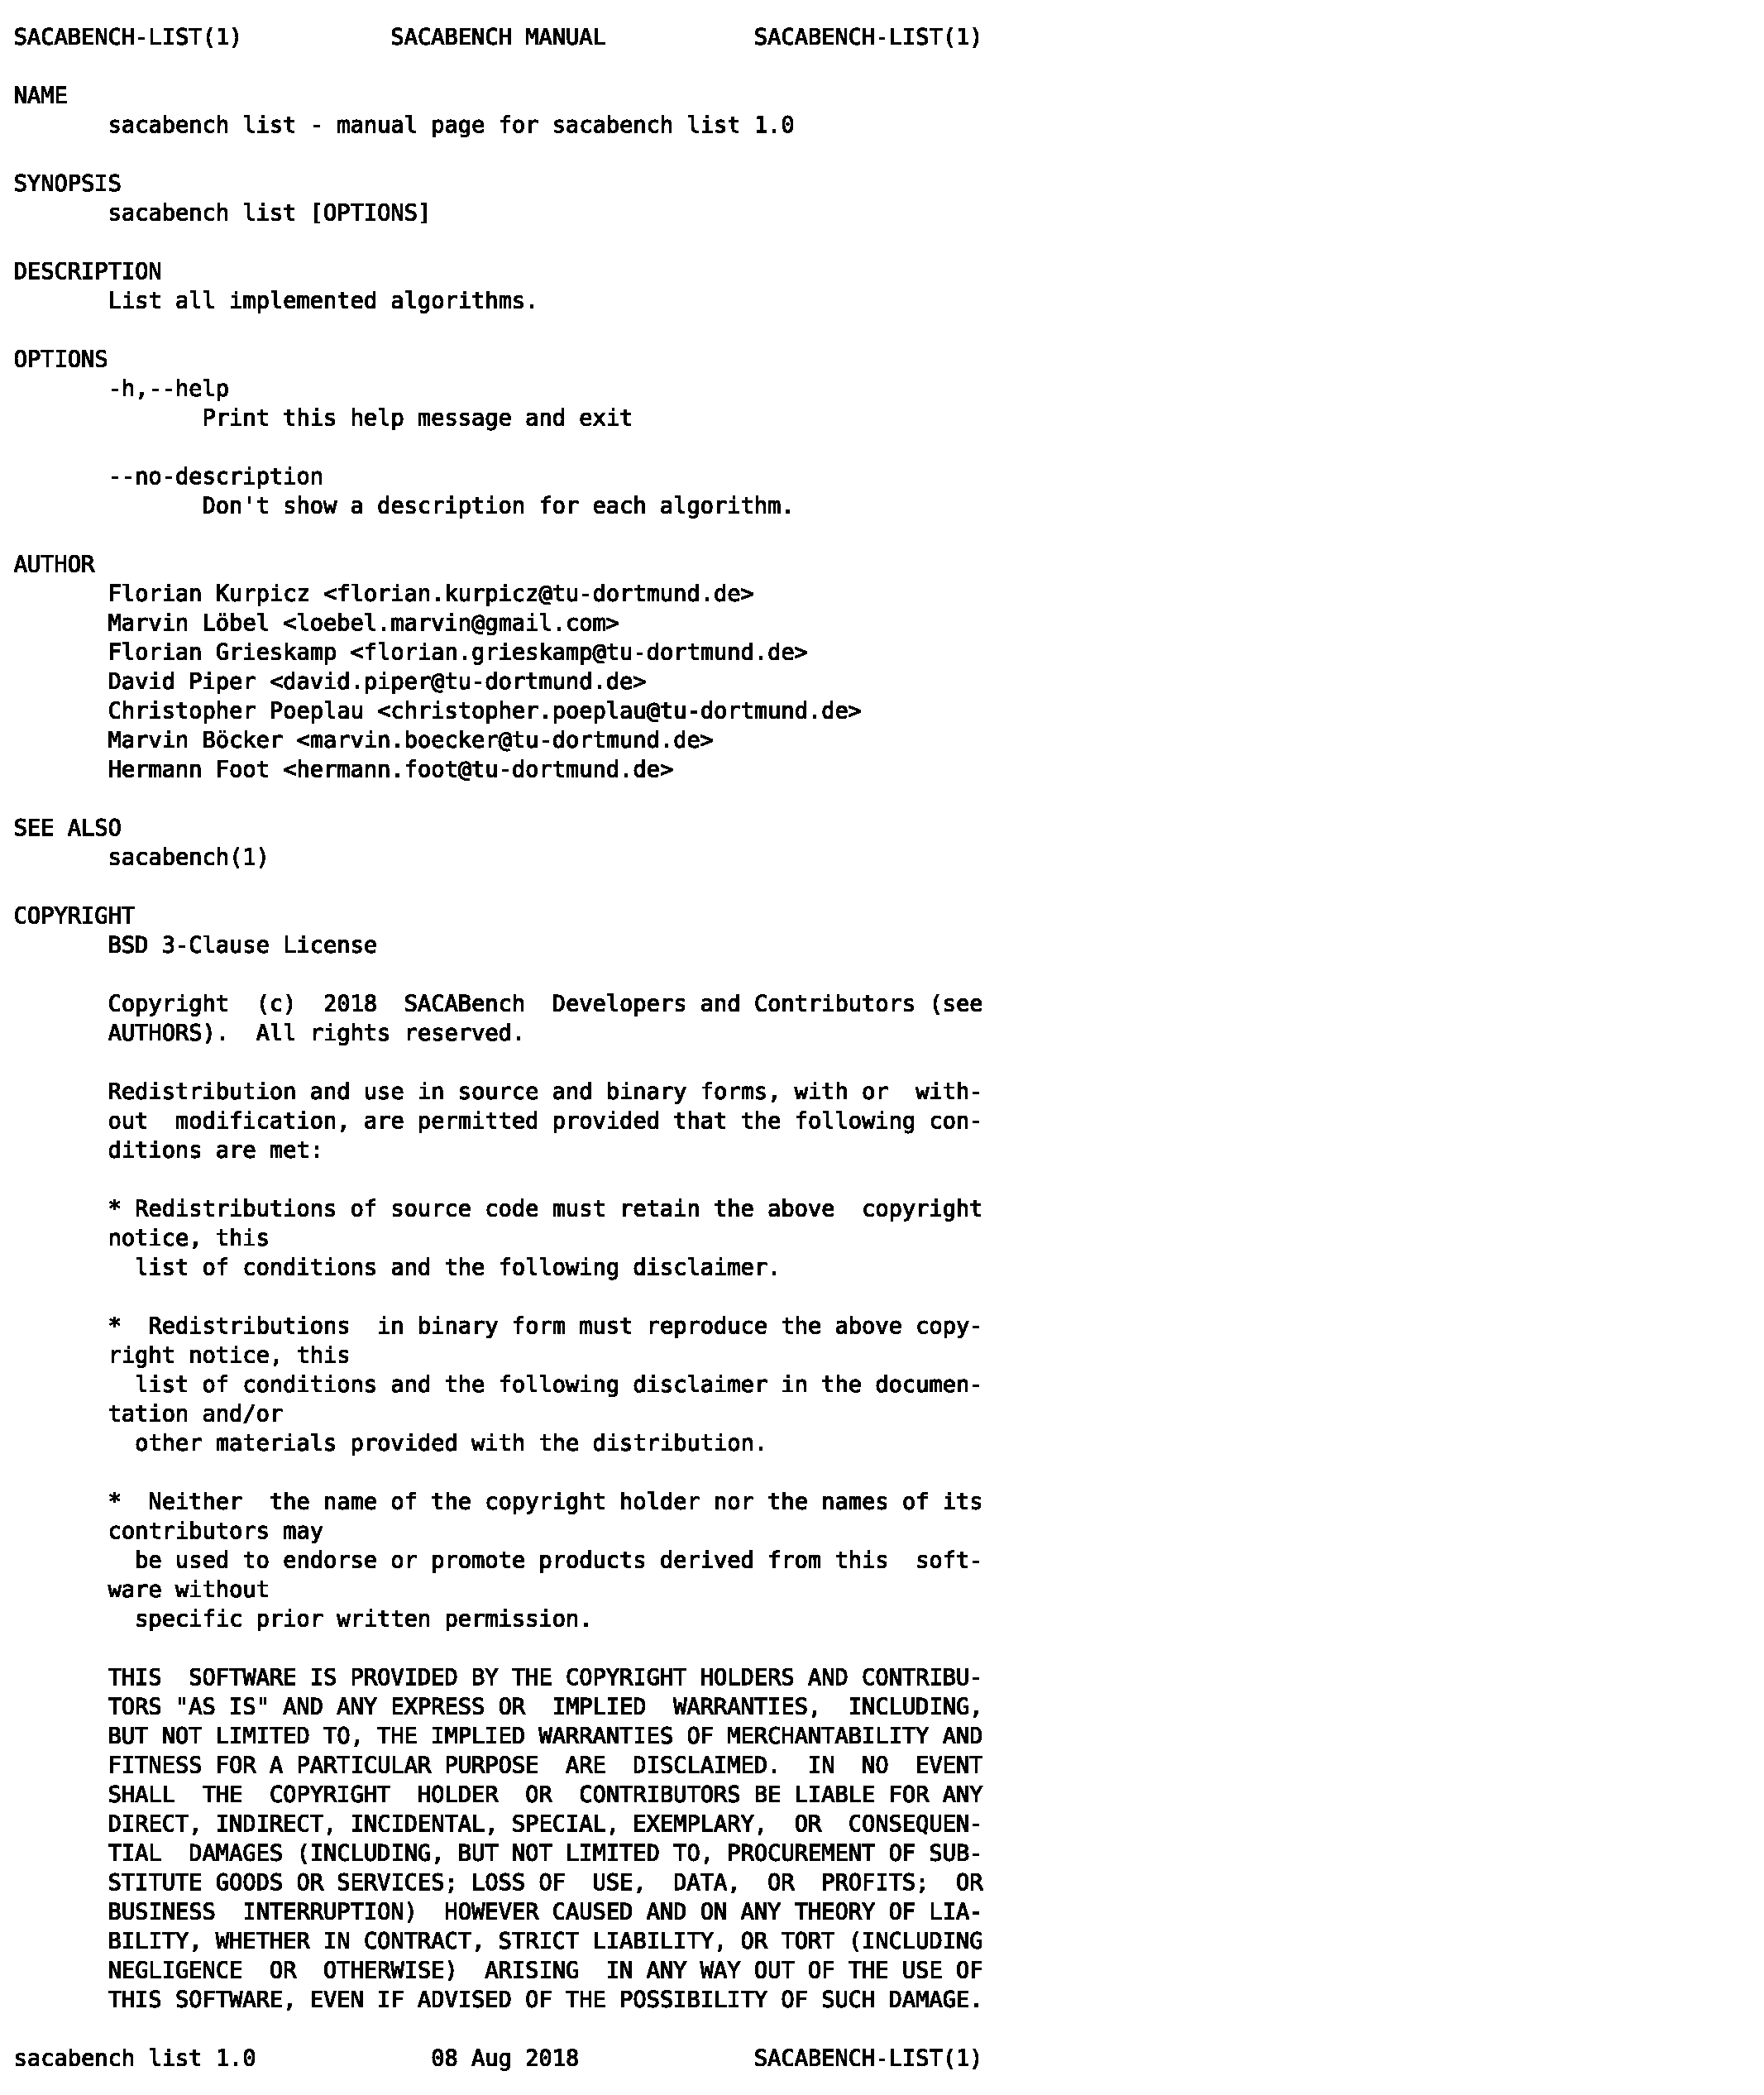
\includegraphics[page=1, viewport=0cm 25cm 20.5cm 26.3cm, clip, width=.5\textwidth]{{kapitel/3_framework/cli/sacabench-list/sacabench-list}.pdf}\\
    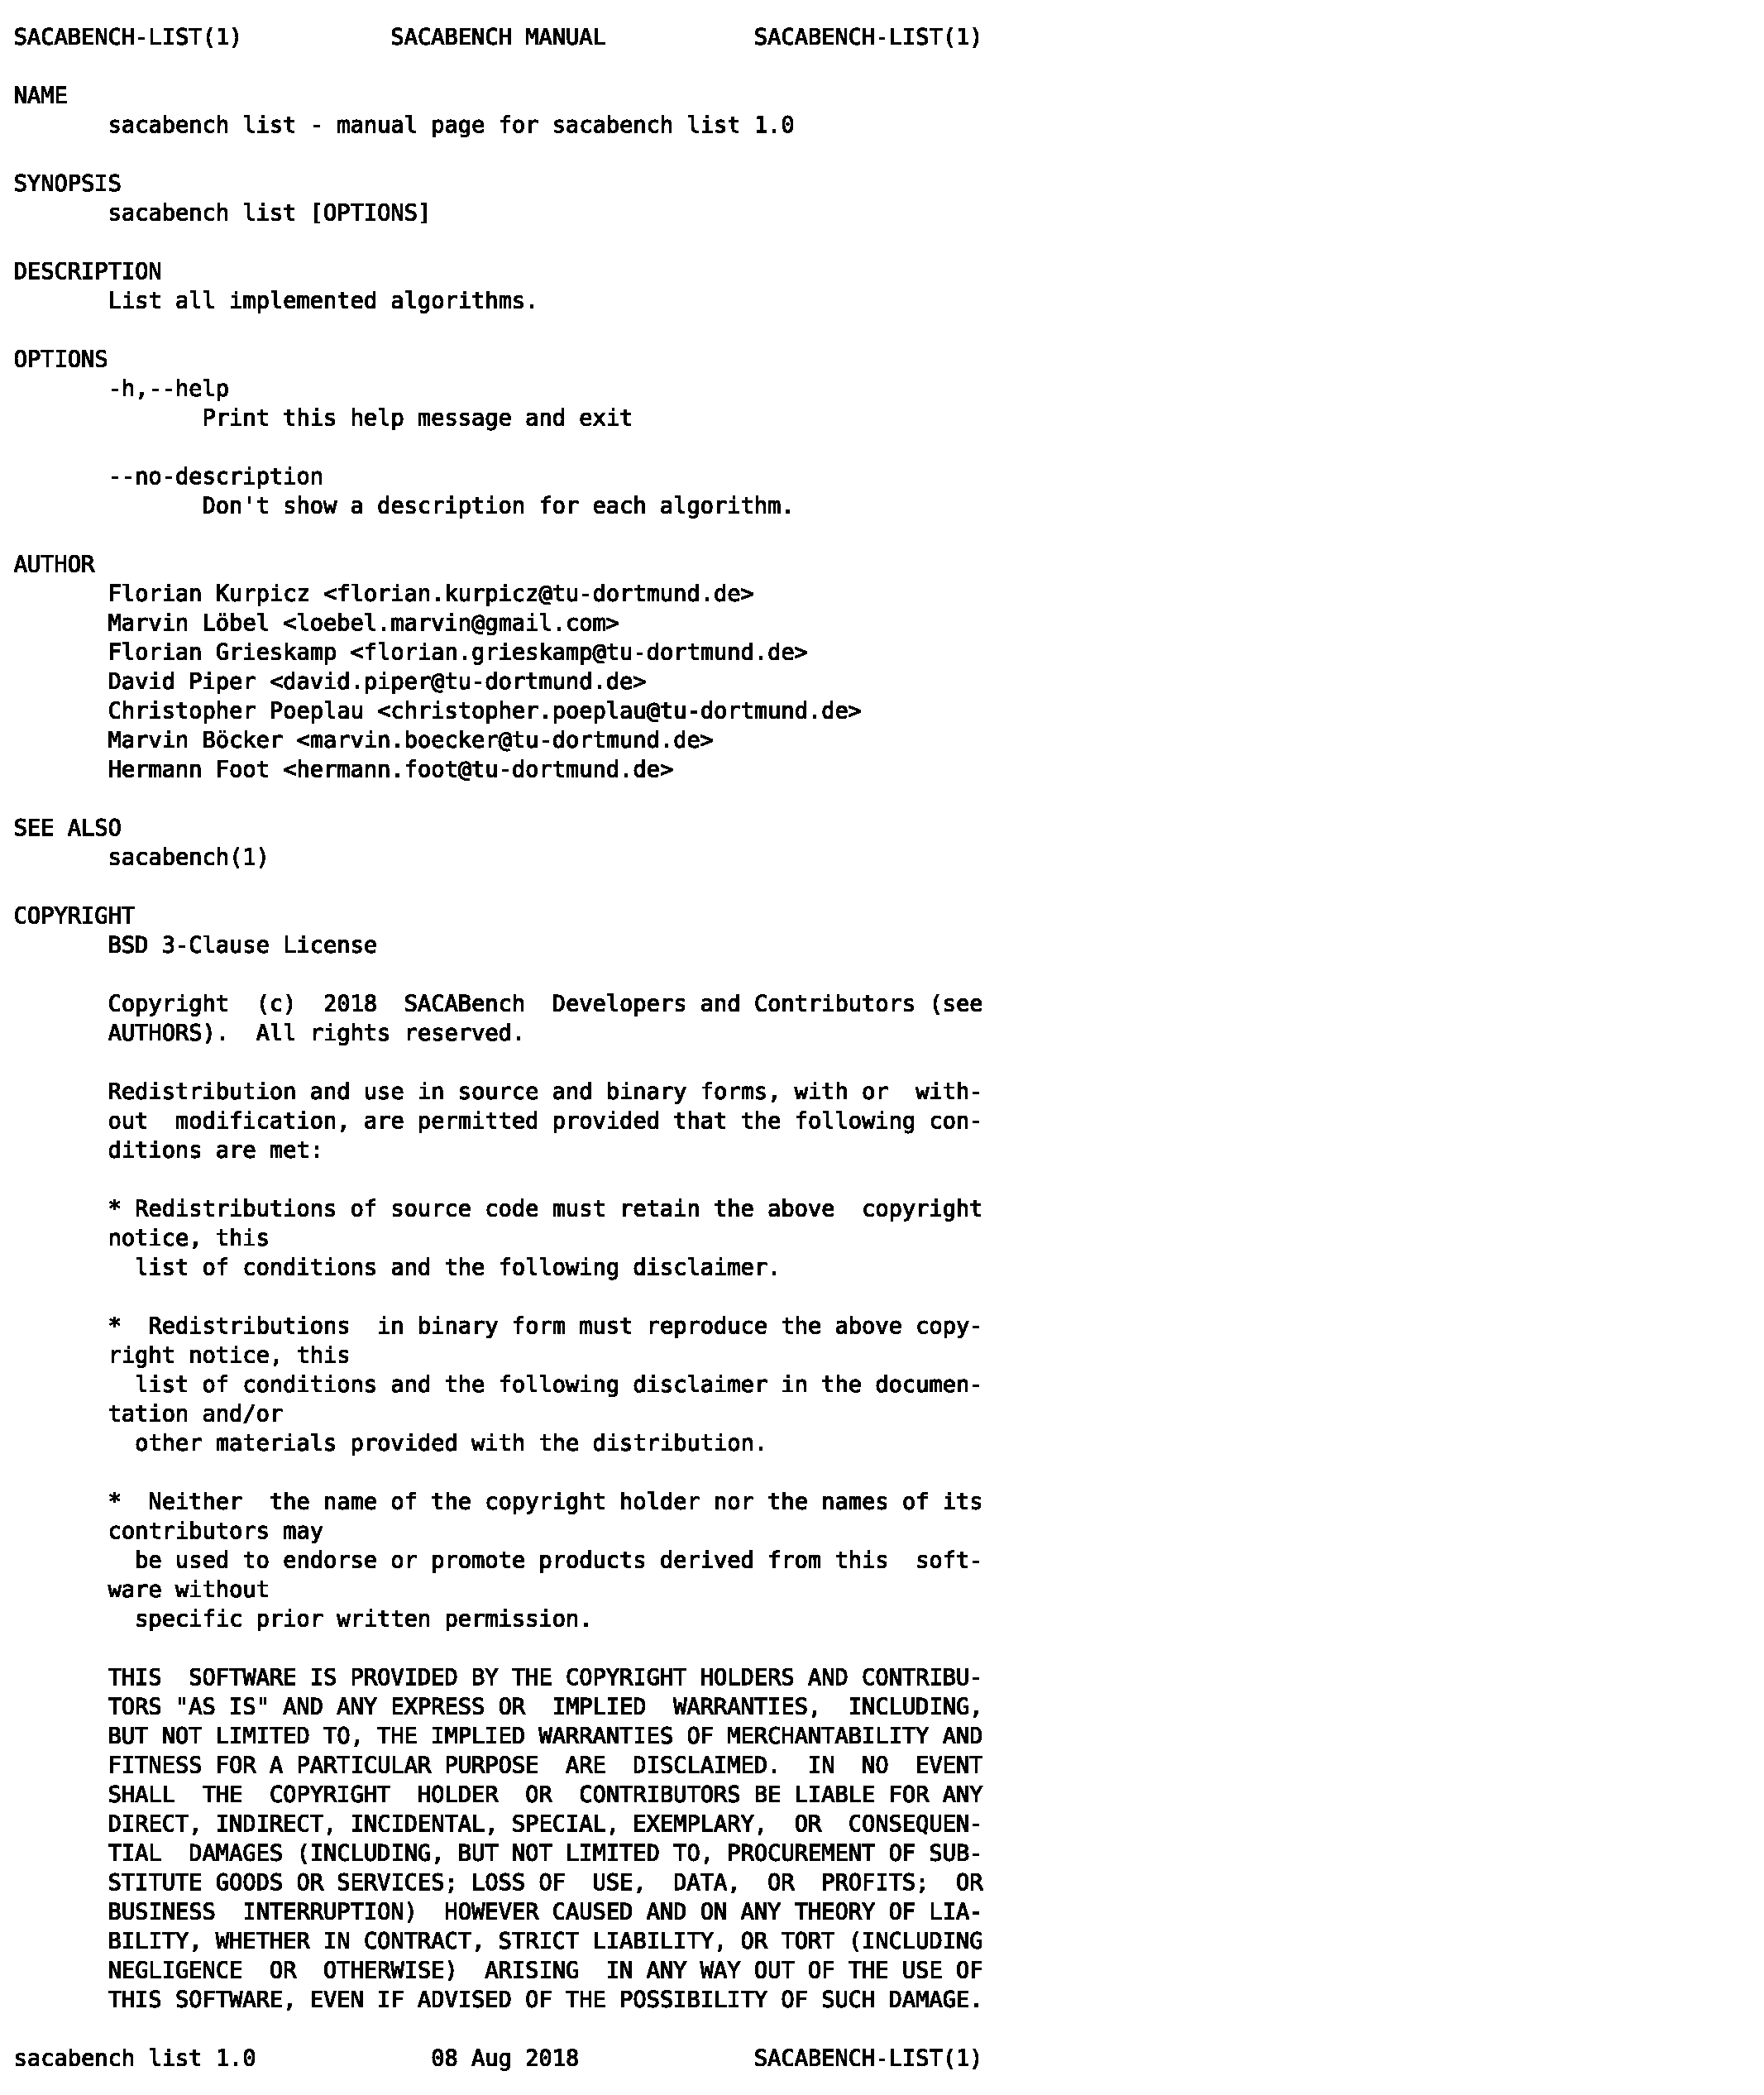
\includegraphics[page=1, viewport=0cm 0cm 20.5cm 1.5cm, clip, width=.5\textwidth]{{kapitel/3_framework/cli/sacabench-list/sacabench-list}.pdf}
    \caption{gekürzte Ausgabe von \texttt{man sacabench list}}
    \label{manpage:sacabench-list}
\end{wrapfigure}
Mit dem Befehl \texttt{sacabench list} können alle verfügbaren Algorithmen aufgelistet werden.
Nach dem Aufruf erscheint eine Liste aller im Rahmen der Projektgruppe implementierten Algorithmen, sowie deren Referenzimplementierungen. Letztere sind in der angegebenen Abkürzung durch \termfont{\_ref} markiert.\par
Über die Option \termfont{-{}-no-description} kann außerdem die Ausgabe der Kurz\-be\-schrei\-bungen unterdrückt werden, sodass nur noch eine Liste aller Kürzel erscheint. Die dort aufgelisteten Kürzel entsprechen den Bezeichnungen der Algorithmen, über die sie vom Framework referenziert werden.\par
}
